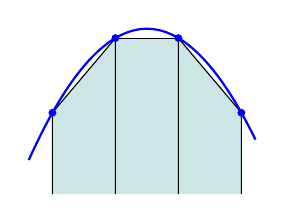
\begin{tikzpicture}[scale=0.6
% ,declare function={f(\x)=-((\x-3)/1.5)^2+3.5;}
]

\pgfmathdeclarefunction{f}{1}{%
    \pgfmathparse{-((#1 - 3) / 1.5)^2 + 3.5}%
}
\coordinate (start) at (.8,{f(.8)});
\coordinate (x0) at (1,{f(1)});
\coordinate (x1) at (1+4/3,{f(1+4/3)});
\coordinate (x2) at (1+8/3,{f(1+8/3)});
\coordinate (x3) at (1+12/3,{f(1+12/3)});
\coordinate (end) at (5.05,{f(5.05)});

\draw[fill=teal!20!white] (1,0)--(1,{f(1)})--(1+4/3,{f(1+4/3)})--(1+4/3,0);
\draw[fill=teal!20!white] (1+4/3,0)--(1+4/3,{f(1+4/3)})--(1+8/3,{f(1+8/3)})--(1+8/3,0);
\draw[fill=teal!20!white] (1+8/3,0)--(1+8/3,{f(1+8/3)})--(5,{f(5)})--(5,0);

\draw[domain=.5:5.3,samples=200,variable=\x,blue,thick] plot ({\x},{f(\x)});                 

\draw[blue,fill=blue] (x0) circle (2pt);    
\draw[blue,fill=blue] (x1) circle (2pt);    
\draw[blue,fill=blue] (x2) circle (2pt);    
\draw[blue,fill=blue] (x3) circle (2pt);  

\end{tikzpicture}